\documentclass[twoside]{book}

% Packages required by doxygen
\usepackage{fixltx2e}
\usepackage{calc}
\usepackage{doxygen}
\usepackage[export]{adjustbox} % also loads graphicx
\usepackage{graphicx}
\usepackage[utf8]{inputenc}
\usepackage{makeidx}
\usepackage{multicol}
\usepackage{multirow}
\PassOptionsToPackage{warn}{textcomp}
\usepackage{textcomp}
\usepackage[nointegrals]{wasysym}
\usepackage[table]{xcolor}

% Font selection
\usepackage[T1]{fontenc}
\usepackage[scaled=.90]{helvet}
\usepackage{courier}
\usepackage{amssymb}
\usepackage{sectsty}
\renewcommand{\familydefault}{\sfdefault}
\allsectionsfont{%
  \fontseries{bc}\selectfont%
  \color{darkgray}%
}
\renewcommand{\DoxyLabelFont}{%
  \fontseries{bc}\selectfont%
  \color{darkgray}%
}
\newcommand{\+}{\discretionary{\mbox{\scriptsize$\hookleftarrow$}}{}{}}

% Page & text layout
\usepackage{geometry}
\geometry{%
  a4paper,%
  top=2.5cm,%
  bottom=2.5cm,%
  left=2.5cm,%
  right=2.5cm%
}
\tolerance=750
\hfuzz=15pt
\hbadness=750
\setlength{\emergencystretch}{15pt}
\setlength{\parindent}{0cm}
\setlength{\parskip}{3ex plus 2ex minus 2ex}
\makeatletter
\renewcommand{\paragraph}{%
  \@startsection{paragraph}{4}{0ex}{-1.0ex}{1.0ex}{%
    \normalfont\normalsize\bfseries\SS@parafont%
  }%
}
\renewcommand{\subparagraph}{%
  \@startsection{subparagraph}{5}{0ex}{-1.0ex}{1.0ex}{%
    \normalfont\normalsize\bfseries\SS@subparafont%
  }%
}
\makeatother

% Headers & footers
\usepackage{fancyhdr}
\pagestyle{fancyplain}
\fancyhead[LE]{\fancyplain{}{\bfseries\thepage}}
\fancyhead[CE]{\fancyplain{}{}}
\fancyhead[RE]{\fancyplain{}{\bfseries\leftmark}}
\fancyhead[LO]{\fancyplain{}{\bfseries\rightmark}}
\fancyhead[CO]{\fancyplain{}{}}
\fancyhead[RO]{\fancyplain{}{\bfseries\thepage}}
\fancyfoot[LE]{\fancyplain{}{}}
\fancyfoot[CE]{\fancyplain{}{}}
\fancyfoot[RE]{\fancyplain{}{\bfseries\scriptsize Generated by Doxygen }}
\fancyfoot[LO]{\fancyplain{}{\bfseries\scriptsize Generated by Doxygen }}
\fancyfoot[CO]{\fancyplain{}{}}
\fancyfoot[RO]{\fancyplain{}{}}
\renewcommand{\footrulewidth}{0.4pt}
\renewcommand{\chaptermark}[1]{%
  \markboth{#1}{}%
}
\renewcommand{\sectionmark}[1]{%
  \markright{\thesection\ #1}%
}

% Indices & bibliography
\usepackage{natbib}
\usepackage[titles]{tocloft}
\setcounter{tocdepth}{3}
\setcounter{secnumdepth}{5}
\makeindex

% Hyperlinks (required, but should be loaded last)
\usepackage{ifpdf}
\ifpdf
  \usepackage[pdftex,pagebackref=true]{hyperref}
\else
  \usepackage[ps2pdf,pagebackref=true]{hyperref}
\fi
\hypersetup{%
  colorlinks=true,%
  linkcolor=blue,%
  citecolor=blue,%
  unicode%
}

% Custom commands
\newcommand{\clearemptydoublepage}{%
  \newpage{\pagestyle{empty}\cleardoublepage}%
}

\usepackage{caption}
\captionsetup{labelsep=space,justification=centering,font={bf},singlelinecheck=off,skip=4pt,position=top}

%===== C O N T E N T S =====

\begin{document}

% Titlepage & ToC
\hypersetup{pageanchor=false,
             bookmarksnumbered=true,
             pdfencoding=unicode
            }
\pagenumbering{alph}
\begin{titlepage}
\vspace*{7cm}
\begin{center}%
{\Large Doxygen\+Generator\+Window \\[1ex]\large 1.\+0.\+0 }\\
\vspace*{1cm}
{\large Generated by Doxygen 1.8.13}\\
\end{center}
\end{titlepage}
\clearemptydoublepage
\pagenumbering{roman}
\tableofcontents
\clearemptydoublepage
\pagenumbering{arabic}
\hypersetup{pageanchor=true}

%--- Begin generated contents ---
\chapter{Doxygen© Generator Window}
\label{md_Assets_DoxygenGeneratorWindow_README}
\Hypertarget{md_Assets_DoxygenGeneratorWindow_README}
\subsection*{Help you to document easily your projects}

This package is very easily to use \+:


\begin{DoxyItemize}
\item in Unity3d Project select menu $>$ide\+Mobi$>$Doxygen© Generator Window
\item select path to Doxygen© \+:
\begin{DoxyItemize}
\item if Doxygen is not installed , follow instructions to download Doxygen for mac\+O\+S© or Windows© at \href{http://www.stack.nl/~dimitri/doxygen/index.html}{\tt http\+://www.\+stack.\+nl/$\sim$dimitri/doxygen/index.\+html}
\end{DoxyItemize}
\item enter informations for your project
\item drag and drop the folder of your scripts (scan is recursive, no panic)
\item select the folder to output the documentation
\item save your config (to restore the next time the save config)
\item {\bfseries generate the documentation}!
\item be happy!
\end{DoxyItemize}

\subsection*{Copyrights}


\begin{DoxyItemize}
\item Copyright © 1997-\/2016 by Dimitri van Heesch. (\href{http://www.stack.nl/~dimitri/doxygen/index.html}{\tt http\+://www.\+stack.\+nl/$\sim$dimitri/doxygen/index.\+html})
\item Copyright © 2017 Apple Inc. (\href{http://www.aplle.com}{\tt http\+://www.\+aplle.\+com})
\item Copyright © 2017 Microsoft (\href{http://www.microsoft.com}{\tt http\+://www.\+microsoft.\+com}) 
\end{DoxyItemize}
\chapter{Modules Index}
\section{Namespace List}
Here is a list of all namespaces with brief descriptions\+:\begin{DoxyCompactList}
\item\contentsline{section}{\hyperlink{namespace_doxygen_generator_window}{Doxygen\+Generator\+Window} }{\pageref{namespace_doxygen_generator_window}}{}
\end{DoxyCompactList}

\chapter{Data Type Index}
\doxysection{Design Unit Hierarchy}
Here is a hierarchical list of all entities\+:\begin{DoxyCompactList}
\item \contentsline{section}{D\+G\+W\+Config}{\pageref{classDoxygenGeneratorWindow_1_1DGWConfig}}{}
\item \contentsline{section}{D\+G\+W\+Config\+List}{\pageref{classDoxygenGeneratorWindow_1_1DGWConfigList}}{}
\item \contentsline{section}{D\+G\+W\+Constants}{\pageref{classDoxygenGeneratorWindow_1_1DGWConstants}}{}
\item \contentsline{section}{D\+G\+W\+Editor\+Menu}{\pageref{classDoxygenGeneratorWindow_1_1DGWEditorMenu}}{}
\item \contentsline{section}{D\+G\+W\+Toolbox}{\pageref{classDoxygenGeneratorWindow_1_1DGWToolbox}}{}
\item \contentsline{section}{D\+G\+W\+Toolbox.\+Thread\+Data}{\pageref{classDoxygenGeneratorWindow_1_1DGWToolbox_1_1ThreadData}}{}
\item Editor\begin{DoxyCompactList}
\item \contentsline{section}{Readme\+Editor}{\pageref{classReadmeEditor}}{}
\end{DoxyCompactList}
\item Editor\+Window\begin{DoxyCompactList}
\item \contentsline{section}{D\+G\+W\+Documentation\+Generator}{\pageref{classDoxygenGeneratorWindow_1_1DGWDocumentationGenerator}}{}
\end{DoxyCompactList}
\item I\+Active\+Build\+Target\+Changed\begin{DoxyCompactList}
\item \contentsline{section}{D\+G\+W\+Macro\+Define}{\pageref{classDoxygenGeneratorWindow_1_1DGWMacroDefine}}{}
\end{DoxyCompactList}
\item Mono\+Behaviour\begin{DoxyCompactList}
\item \contentsline{section}{Simple\+Camera\+Controller}{\pageref{classUnityTemplateProjects_1_1SimpleCameraController}}{}
\end{DoxyCompactList}
\item \contentsline{section}{Readme.\+Section}{\pageref{classReadme_1_1Section}}{}
\item Scriptable\+Object\begin{DoxyCompactList}
\item \contentsline{section}{D\+G\+W\+Find\+Package}{\pageref{classDoxygenGeneratorWindow_1_1DGWFindPackage}}{}
\item \contentsline{section}{Readme}{\pageref{classReadme}}{}
\end{DoxyCompactList}
\item \contentsline{section}{Simple\+Camera\+Controller.\+Camera\+State}{\pageref{classUnityTemplateProjects_1_1SimpleCameraController_1_1CameraState}}{}
\end{DoxyCompactList}

\chapter{Data Type Index}
\doxysection{Data Types List}
Here are the data types with brief descriptions\+:\begin{DoxyCompactList}
\item\contentsline{section}{\mbox{\hyperlink{classDoxygenGeneratorWindow_1_1DGWConfig}{D\+G\+W\+Config}} \\*D\+GW config reccord your config... it\textquotesingle{}s enough! }{\pageref{classDoxygenGeneratorWindow_1_1DGWConfig}}{}
\item\contentsline{section}{\mbox{\hyperlink{classDoxygenGeneratorWindow_1_1DGWConfigList}{D\+G\+W\+Config\+List}} \\*D\+GW config List reccord your config! }{\pageref{classDoxygenGeneratorWindow_1_1DGWConfigList}}{}
\item\contentsline{section}{\mbox{\hyperlink{classDoxygenGeneratorWindow_1_1DGWConstants}{D\+G\+W\+Constants}} }{\pageref{classDoxygenGeneratorWindow_1_1DGWConstants}}{}
\item\contentsline{section}{\mbox{\hyperlink{classDoxygenGeneratorWindow_1_1DGWDocumentationGenerator}{D\+G\+W\+Documentation\+Generator}} }{\pageref{classDoxygenGeneratorWindow_1_1DGWDocumentationGenerator}}{}
\item\contentsline{section}{\mbox{\hyperlink{classDoxygenGeneratorWindow_1_1DGWEditorMenu}{D\+G\+W\+Editor\+Menu}} \\*D\+GW editor menu }{\pageref{classDoxygenGeneratorWindow_1_1DGWEditorMenu}}{}
\item\contentsline{section}{\mbox{\hyperlink{classDoxygenGeneratorWindow_1_1DGWFindPackage}{D\+G\+W\+Find\+Package}} \\*Find package path class. Use the Scriptable\+Object to find the path of this package }{\pageref{classDoxygenGeneratorWindow_1_1DGWFindPackage}}{}
\item\contentsline{section}{\mbox{\hyperlink{classDoxygenGeneratorWindow_1_1DGWMacroDefine}{D\+G\+W\+Macro\+Define}} \\*Macro define can find if k\+Macro is set in the settings and add it if necessary. This class auto run at build project. You can use k\+Macro in precompile definition }{\pageref{classDoxygenGeneratorWindow_1_1DGWMacroDefine}}{}
\item\contentsline{section}{\mbox{\hyperlink{classDoxygenGeneratorWindow_1_1DGWToolbox}{D\+G\+W\+Toolbox}} }{\pageref{classDoxygenGeneratorWindow_1_1DGWToolbox}}{}
\item\contentsline{section}{\mbox{\hyperlink{classDoxygenGeneratorWindow_1_1DGWToolbox_1_1ThreadData}{D\+G\+W\+Toolbox.\+Thread\+Data}} }{\pageref{classDoxygenGeneratorWindow_1_1DGWToolbox_1_1ThreadData}}{}
\item\contentsline{section}{\mbox{\hyperlink{classReadme}{Readme}} }{\pageref{classReadme}}{}
\item\contentsline{section}{\mbox{\hyperlink{classReadme_1_1Section}{Readme.\+Section}} }{\pageref{classReadme_1_1Section}}{}
\item\contentsline{section}{\mbox{\hyperlink{classReadmeEditor}{Readme\+Editor}} }{\pageref{classReadmeEditor}}{}
\item\contentsline{section}{\mbox{\hyperlink{classUnityTemplateProjects_1_1SimpleCameraController}{Simple\+Camera\+Controller}} }{\pageref{classUnityTemplateProjects_1_1SimpleCameraController}}{}
\item\contentsline{section}{\mbox{\hyperlink{classUnityTemplateProjects_1_1SimpleCameraController_1_1CameraState}{Simple\+Camera\+Controller.\+Camera\+State}} }{\pageref{classUnityTemplateProjects_1_1SimpleCameraController_1_1CameraState}}{}
\end{DoxyCompactList}

\chapter{File Index}
\section{File List}
Here is a list of all files with brief descriptions\+:\begin{DoxyCompactList}
\item\contentsline{section}{Assets/\+Doxygen\+Generator\+Window/\hyperlink{_d_g_w_constants_8cs}{D\+G\+W\+Constants.\+cs} }{\pageref{_d_g_w_constants_8cs}}{}
\item\contentsline{section}{Assets/\+Doxygen\+Generator\+Window/\hyperlink{_d_g_w_documentation_generator_8cs}{D\+G\+W\+Documentation\+Generator.\+cs} }{\pageref{_d_g_w_documentation_generator_8cs}}{}
\end{DoxyCompactList}

\chapter{Module Documentation}
\hypertarget{namespaceDoxygenGeneratorWindow}{}\doxysection{Doxygen\+Generator\+Window Namespace Reference}
\label{namespaceDoxygenGeneratorWindow}\index{DoxygenGeneratorWindow@{DoxygenGeneratorWindow}}
\doxysubsection*{Data Structures}
\begin{DoxyCompactItemize}
\item 
class \mbox{\hyperlink{classDoxygenGeneratorWindow_1_1DGWConfig}{D\+G\+W\+Config}}
\begin{DoxyCompactList}\small\item\em D\+GW config reccord your config... it\textquotesingle{}s enough! \end{DoxyCompactList}\item 
class \mbox{\hyperlink{classDoxygenGeneratorWindow_1_1DGWConfigList}{D\+G\+W\+Config\+List}}
\begin{DoxyCompactList}\small\item\em D\+GW config List reccord your config! \end{DoxyCompactList}\item 
class \mbox{\hyperlink{classDoxygenGeneratorWindow_1_1DGWConstants}{D\+G\+W\+Constants}}
\item 
class \mbox{\hyperlink{classDoxygenGeneratorWindow_1_1DGWDocumentationGenerator}{D\+G\+W\+Documentation\+Generator}}
\item 
class \mbox{\hyperlink{classDoxygenGeneratorWindow_1_1DGWEditorMenu}{D\+G\+W\+Editor\+Menu}}
\begin{DoxyCompactList}\small\item\em D\+GW editor menu. \end{DoxyCompactList}\item 
class \mbox{\hyperlink{classDoxygenGeneratorWindow_1_1DGWFindPackage}{D\+G\+W\+Find\+Package}}
\begin{DoxyCompactList}\small\item\em Find package path class. Use the Scriptable\+Object to find the path of this package \end{DoxyCompactList}\item 
class \mbox{\hyperlink{classDoxygenGeneratorWindow_1_1DGWMacroDefine}{D\+G\+W\+Macro\+Define}}
\begin{DoxyCompactList}\small\item\em Macro define can find if k\+Macro is set in the settings and add it if necessary. This class auto run at build project. You can use k\+Macro in precompile definition. \end{DoxyCompactList}\item 
class \mbox{\hyperlink{classDoxygenGeneratorWindow_1_1DGWToolbox}{D\+G\+W\+Toolbox}}
\end{DoxyCompactItemize}
\doxysubsection*{Enumerations}


\doxysubsection{Enumeration Type Documentation}
\mbox{\Hypertarget{namespaceDoxygenGeneratorWindow_a0f776a0aa7d33a4f3663cccf4fdd9ecd}\label{namespaceDoxygenGeneratorWindow_a0f776a0aa7d33a4f3663cccf4fdd9ecd}} 
\index{DoxygenGeneratorWindow@{DoxygenGeneratorWindow}!DGWTools@{DGWTools}}
\index{DGWTools@{DGWTools}!DoxygenGeneratorWindow@{DoxygenGeneratorWindow}}
\doxysubsubsection{\texorpdfstring{DGWTools}{DGWTools}}
{\footnotesize\ttfamily enum D\+G\+W\+Tools \+: int\hspace{0.3cm}{\ttfamily [strong]}}



D\+GW Documentation generator is a class to generate the documentation by Doxygen automatically After reading comparison at \href{https://en.wikipedia.org/wiki/Comparison_of_documentation_generators}{\texttt{ https\+://en.\+wikipedia.\+org/wiki/\+Comparison\+\_\+of\+\_\+documentation\+\_\+generators}} the challengers for c\# with output H\+T\+ML are ... 


\begin{DoxyItemize}
\item Document! X (eliminated \+: no mac\+OS, no linux)
\item Doxygen
\item Natural Docs (partial P\+HP ...)
\item N\+Doc (eliminated \+: no read text as input!)
\item Visual Expert (eliminated \+: no mac\+OS, no linux)
\item V\+Sdocman (eliminated \+: no mac\+OS, no linux) We decided to use Doxygen beacuse it\textquotesingle{}s the most easy to use for a proof of concept. We will propose Natural Docs later, because the library is not really usable on macosx
\end{DoxyItemize}\begin{DoxyEnumFields}{Enumerator}
\raisebox{\heightof{T}}[0pt][0pt]{\index{Doxygen@{Doxygen}!DoxygenGeneratorWindow@{DoxygenGeneratorWindow}}\index{DoxygenGeneratorWindow@{DoxygenGeneratorWindow}!Doxygen@{Doxygen}}}\mbox{\Hypertarget{namespaceDoxygenGeneratorWindow_a0f776a0aa7d33a4f3663cccf4fdd9ecda7f20b283fe8e6e7416c8090e0660c2fe}\label{namespaceDoxygenGeneratorWindow_a0f776a0aa7d33a4f3663cccf4fdd9ecda7f20b283fe8e6e7416c8090e0660c2fe}} 
Doxygen&\\
\hline

\end{DoxyEnumFields}

\chapter{Data Type Documentation}
\hypertarget{classDoxygenGeneratorWindow_1_1DGWConfig}{}\doxysection{D\+G\+W\+Config Class Reference}
\label{classDoxygenGeneratorWindow_1_1DGWConfig}\index{DGWConfig@{DGWConfig}}


D\+GW config reccord your config... it\textquotesingle{}s enough!  


\doxysubsection*{Public Member Functions}
\doxysubsection*{Data Fields}


\doxysubsection{Detailed Description}
D\+GW config reccord your config... it\textquotesingle{}s enough! 



\doxysubsection{Constructor \& Destructor Documentation}
\mbox{\Hypertarget{classDoxygenGeneratorWindow_1_1DGWConfig_a111475dc4f19bf6be8e22f68ba7c483f}\label{classDoxygenGeneratorWindow_1_1DGWConfig_a111475dc4f19bf6be8e22f68ba7c483f}} 
\index{DGWConfig@{DGWConfig}!DGWConfig@{DGWConfig}}
\index{DGWConfig@{DGWConfig}!DGWConfig@{DGWConfig}}
\doxysubsubsection{\texorpdfstring{DGWConfig()}{DGWConfig()}}
{\footnotesize\ttfamily D\+G\+W\+Config (\begin{DoxyParamCaption}{ }\end{DoxyParamCaption})}



\doxysubsection{Member Function Documentation}
\mbox{\Hypertarget{classDoxygenGeneratorWindow_1_1DGWConfig_a25e1ad80533fbf1ddec9785e5f5662ae}\label{classDoxygenGeneratorWindow_1_1DGWConfig_a25e1ad80533fbf1ddec9785e5f5662ae}} 
\index{DGWConfig@{DGWConfig}!EmptyFill@{EmptyFill}}
\index{EmptyFill@{EmptyFill}!DGWConfig@{DGWConfig}}
\doxysubsubsection{\texorpdfstring{EmptyFill()}{EmptyFill()}}
{\footnotesize\ttfamily void Empty\+Fill (\begin{DoxyParamCaption}{ }\end{DoxyParamCaption})}

\mbox{\Hypertarget{classDoxygenGeneratorWindow_1_1DGWConfig_a4afbe4efb2ce34d4e3ea871a703d12b8}\label{classDoxygenGeneratorWindow_1_1DGWConfig_a4afbe4efb2ce34d4e3ea871a703d12b8}} 
\index{DGWConfig@{DGWConfig}!FolderOutputAbsolute@{FolderOutputAbsolute}}
\index{FolderOutputAbsolute@{FolderOutputAbsolute}!DGWConfig@{DGWConfig}}
\doxysubsubsection{\texorpdfstring{FolderOutputAbsolute()}{FolderOutputAbsolute()}}
{\footnotesize\ttfamily string Folder\+Output\+Absolute (\begin{DoxyParamCaption}{ }\end{DoxyParamCaption})}

\mbox{\Hypertarget{classDoxygenGeneratorWindow_1_1DGWConfig_a31730f143952e39be16d00e588e3cc3f}\label{classDoxygenGeneratorWindow_1_1DGWConfig_a31730f143952e39be16d00e588e3cc3f}} 
\index{DGWConfig@{DGWConfig}!SetFolderOutputAbsolute@{SetFolderOutputAbsolute}}
\index{SetFolderOutputAbsolute@{SetFolderOutputAbsolute}!DGWConfig@{DGWConfig}}
\doxysubsubsection{\texorpdfstring{SetFolderOutputAbsolute()}{SetFolderOutputAbsolute()}}
{\footnotesize\ttfamily void Set\+Folder\+Output\+Absolute (\begin{DoxyParamCaption}\item[{string}]{s\+Absolute\+Path }\end{DoxyParamCaption})}



\doxysubsection{Field Documentation}
\mbox{\Hypertarget{classDoxygenGeneratorWindow_1_1DGWConfig_a5c3dcfc1c2400906e7f18ed049543dde}\label{classDoxygenGeneratorWindow_1_1DGWConfig_a5c3dcfc1c2400906e7f18ed049543dde}} 
\index{DGWConfig@{DGWConfig}!ALPHABETICAL\_INDEX@{ALPHABETICAL\_INDEX}}
\index{ALPHABETICAL\_INDEX@{ALPHABETICAL\_INDEX}!DGWConfig@{DGWConfig}}
\doxysubsubsection{\texorpdfstring{ALPHABETICAL\_INDEX}{ALPHABETICAL\_INDEX}}
{\footnotesize\ttfamily bool A\+L\+P\+H\+A\+B\+E\+T\+I\+C\+A\+L\+\_\+\+I\+N\+D\+EX = true}



Is analyze is A\+L\+P\+H\+A\+B\+E\+T\+I\+C\+A\+L\+\_\+\+I\+N\+D\+EX or not?. 

\mbox{\Hypertarget{classDoxygenGeneratorWindow_1_1DGWConfig_a472d53f7c4288664428e563eecc4ade2}\label{classDoxygenGeneratorWindow_1_1DGWConfig_a472d53f7c4288664428e563eecc4ade2}} 
\index{DGWConfig@{DGWConfig}!FolderName@{FolderName}}
\index{FolderName@{FolderName}!DGWConfig@{DGWConfig}}
\doxysubsubsection{\texorpdfstring{FolderName}{FolderName}}
{\footnotesize\ttfamily string Folder\+Name = \char`\"{}\char`\"{}}



The name of the folder to analyze. 

\mbox{\Hypertarget{classDoxygenGeneratorWindow_1_1DGWConfig_a41baab1251054ddbdcca9996e49c2ca9}\label{classDoxygenGeneratorWindow_1_1DGWConfig_a41baab1251054ddbdcca9996e49c2ca9}} 
\index{DGWConfig@{DGWConfig}!FolderOutput@{FolderOutput}}
\index{FolderOutput@{FolderOutput}!DGWConfig@{DGWConfig}}
\doxysubsubsection{\texorpdfstring{FolderOutput}{FolderOutput}}
{\footnotesize\ttfamily string Folder\+Output = \char`\"{}\char`\"{}}



The folder to output the documentation. 

\mbox{\Hypertarget{classDoxygenGeneratorWindow_1_1DGWConfig_ac4c8e61a0381850552df0a7a5d8588bf}\label{classDoxygenGeneratorWindow_1_1DGWConfig_ac4c8e61a0381850552df0a7a5d8588bf}} 
\index{DGWConfig@{DGWConfig}!GenerateDocSet@{GenerateDocSet}}
\index{GenerateDocSet@{GenerateDocSet}!DGWConfig@{DGWConfig}}
\doxysubsubsection{\texorpdfstring{GenerateDocSet}{GenerateDocSet}}
{\footnotesize\ttfamily bool Generate\+Doc\+Set = false}



The generate Doc set. 

\mbox{\Hypertarget{classDoxygenGeneratorWindow_1_1DGWConfig_a7574a7d4639ff10e9e6b209094857098}\label{classDoxygenGeneratorWindow_1_1DGWConfig_a7574a7d4639ff10e9e6b209094857098}} 
\index{DGWConfig@{DGWConfig}!GenerateHTML@{GenerateHTML}}
\index{GenerateHTML@{GenerateHTML}!DGWConfig@{DGWConfig}}
\doxysubsubsection{\texorpdfstring{GenerateHTML}{GenerateHTML}}
{\footnotesize\ttfamily bool Generate\+H\+T\+ML = true}



The generate H\+T\+ML Doc. 

\mbox{\Hypertarget{classDoxygenGeneratorWindow_1_1DGWConfig_ae17963bf713651d1a847100f5772ff31}\label{classDoxygenGeneratorWindow_1_1DGWConfig_ae17963bf713651d1a847100f5772ff31}} 
\index{DGWConfig@{DGWConfig}!GenerateLatex@{GenerateLatex}}
\index{GenerateLatex@{GenerateLatex}!DGWConfig@{DGWConfig}}
\doxysubsubsection{\texorpdfstring{GenerateLatex}{GenerateLatex}}
{\footnotesize\ttfamily bool Generate\+Latex = false}



The generate latex Doc. 

\mbox{\Hypertarget{classDoxygenGeneratorWindow_1_1DGWConfig_ae77c5b908955768f409b28fbfdfabb86}\label{classDoxygenGeneratorWindow_1_1DGWConfig_ae77c5b908955768f409b28fbfdfabb86}} 
\index{DGWConfig@{DGWConfig}!GenerateRTF@{GenerateRTF}}
\index{GenerateRTF@{GenerateRTF}!DGWConfig@{DGWConfig}}
\doxysubsubsection{\texorpdfstring{GenerateRTF}{GenerateRTF}}
{\footnotesize\ttfamily bool Generate\+R\+TF = false}



The generate R\+TF Doc. 

\mbox{\Hypertarget{classDoxygenGeneratorWindow_1_1DGWConfig_a3bfb001a8099baeb6ec6345ebccd1a9d}\label{classDoxygenGeneratorWindow_1_1DGWConfig_a3bfb001a8099baeb6ec6345ebccd1a9d}} 
\index{DGWConfig@{DGWConfig}!GenerateXML@{GenerateXML}}
\index{GenerateXML@{GenerateXML}!DGWConfig@{DGWConfig}}
\doxysubsubsection{\texorpdfstring{GenerateXML}{GenerateXML}}
{\footnotesize\ttfamily bool Generate\+X\+ML = false}



The generate X\+ML Doc. 

\mbox{\Hypertarget{classDoxygenGeneratorWindow_1_1DGWConfig_ad7059e1c947d816aa5052372ef376581}\label{classDoxygenGeneratorWindow_1_1DGWConfig_ad7059e1c947d816aa5052372ef376581}} 
\index{DGWConfig@{DGWConfig}!HTMLColor@{HTMLColor}}
\index{HTMLColor@{HTMLColor}!DGWConfig@{DGWConfig}}
\doxysubsubsection{\texorpdfstring{HTMLColor}{HTMLColor}}
{\footnotesize\ttfamily Color H\+T\+M\+L\+Color = Color.\+gray}



The tint color of the H\+T\+ML doc. 

\mbox{\Hypertarget{classDoxygenGeneratorWindow_1_1DGWConfig_a98e220d2aa58ce620449040f90e971be}\label{classDoxygenGeneratorWindow_1_1DGWConfig_a98e220d2aa58ce620449040f90e971be}} 
\index{DGWConfig@{DGWConfig}!ProjectLogo@{ProjectLogo}}
\index{ProjectLogo@{ProjectLogo}!DGWConfig@{DGWConfig}}
\doxysubsubsection{\texorpdfstring{ProjectLogo}{ProjectLogo}}
{\footnotesize\ttfamily string Project\+Logo = \char`\"{}\char`\"{}}



The logo for project. 

\mbox{\Hypertarget{classDoxygenGeneratorWindow_1_1DGWConfig_a3fe78671836fb8f22d63f63e0e7865ae}\label{classDoxygenGeneratorWindow_1_1DGWConfig_a3fe78671836fb8f22d63f63e0e7865ae}} 
\index{DGWConfig@{DGWConfig}!ProjectName@{ProjectName}}
\index{ProjectName@{ProjectName}!DGWConfig@{DGWConfig}}
\doxysubsubsection{\texorpdfstring{ProjectName}{ProjectName}}
{\footnotesize\ttfamily string Project\+Name = \char`\"{}\char`\"{}}



The name of the project. 

\mbox{\Hypertarget{classDoxygenGeneratorWindow_1_1DGWConfig_aad02a5539e6fa6b8ca610ac10bc46eca}\label{classDoxygenGeneratorWindow_1_1DGWConfig_aad02a5539e6fa6b8ca610ac10bc46eca}} 
\index{DGWConfig@{DGWConfig}!ProjectSynopsis@{ProjectSynopsis}}
\index{ProjectSynopsis@{ProjectSynopsis}!DGWConfig@{DGWConfig}}
\doxysubsubsection{\texorpdfstring{ProjectSynopsis}{ProjectSynopsis}}
{\footnotesize\ttfamily string Project\+Synopsis = \char`\"{}\char`\"{}}



The project synopsis. 

\mbox{\Hypertarget{classDoxygenGeneratorWindow_1_1DGWConfig_a15a911eb7e938cf68cff61be8f095c9b}\label{classDoxygenGeneratorWindow_1_1DGWConfig_a15a911eb7e938cf68cff61be8f095c9b}} 
\index{DGWConfig@{DGWConfig}!ProjectVersion@{ProjectVersion}}
\index{ProjectVersion@{ProjectVersion}!DGWConfig@{DGWConfig}}
\doxysubsubsection{\texorpdfstring{ProjectVersion}{ProjectVersion}}
{\footnotesize\ttfamily string Project\+Version = \char`\"{}\char`\"{}}



The project version. 

\mbox{\Hypertarget{classDoxygenGeneratorWindow_1_1DGWConfig_a087d066fb97182b1ec164e5103493c9b}\label{classDoxygenGeneratorWindow_1_1DGWConfig_a087d066fb97182b1ec164e5103493c9b}} 
\index{DGWConfig@{DGWConfig}!Recursive@{Recursive}}
\index{Recursive@{Recursive}!DGWConfig@{DGWConfig}}
\doxysubsubsection{\texorpdfstring{Recursive}{Recursive}}
{\footnotesize\ttfamily bool Recursive = true}



Is analyze is recursive or not?. 

\mbox{\Hypertarget{classDoxygenGeneratorWindow_1_1DGWConfig_ac5b6002c3cdbbb1cc5911b91f34b1865}\label{classDoxygenGeneratorWindow_1_1DGWConfig_ac5b6002c3cdbbb1cc5911b91f34b1865}} 
\index{DGWConfig@{DGWConfig}!UseTools@{UseTools}}
\index{UseTools@{UseTools}!DGWConfig@{DGWConfig}}
\doxysubsubsection{\texorpdfstring{UseTools}{UseTools}}
{\footnotesize\ttfamily \mbox{\hyperlink{namespaceDoxygenGeneratorWindow_a0f776a0aa7d33a4f3663cccf4fdd9ecd}{D\+G\+W\+Tools}} Use\+Tools = \mbox{\hyperlink{namespaceDoxygenGeneratorWindow_a0f776a0aa7d33a4f3663cccf4fdd9ecda7f20b283fe8e6e7416c8090e0660c2fe}{D\+G\+W\+Tools.\+Doxygen}}}



The documentation for this class was generated from the following file\+:\begin{DoxyCompactItemize}
\item 
Assets/\+Doxygen\+Generator\+Window/\+Scripts/\+Editor/\mbox{\hyperlink{DGWConfig_8cs}{D\+G\+W\+Config.\+cs}}\end{DoxyCompactItemize}

\hypertarget{classDoxygenGeneratorWindow_1_1DGWConstants}{}\section{D\+G\+W\+Constants Class Reference}
\label{classDoxygenGeneratorWindow_1_1DGWConstants}\index{D\+G\+W\+Constants@{D\+G\+W\+Constants}}
\subsection*{Data Fields}


\subsection{Field Documentation}
\mbox{\Hypertarget{classDoxygenGeneratorWindow_1_1DGWConstants_a3072bfa003c609fe44c1ad1105026305}\label{classDoxygenGeneratorWindow_1_1DGWConstants_a3072bfa003c609fe44c1ad1105026305}} 
\index{Doxygen\+Generator\+Window\+::\+D\+G\+W\+Constants@{Doxygen\+Generator\+Window\+::\+D\+G\+W\+Constants}!K\+\_\+\+A\+L\+E\+R\+T\+\_\+\+I\+D\+E\+M\+O\+B\+I\+\_\+\+D\+O\+C\+\_\+\+H\+T\+TP@{K\+\_\+\+A\+L\+E\+R\+T\+\_\+\+I\+D\+E\+M\+O\+B\+I\+\_\+\+D\+O\+C\+\_\+\+H\+T\+TP}}
\index{K\+\_\+\+A\+L\+E\+R\+T\+\_\+\+I\+D\+E\+M\+O\+B\+I\+\_\+\+D\+O\+C\+\_\+\+H\+T\+TP@{K\+\_\+\+A\+L\+E\+R\+T\+\_\+\+I\+D\+E\+M\+O\+B\+I\+\_\+\+D\+O\+C\+\_\+\+H\+T\+TP}!Doxygen\+Generator\+Window\+::\+D\+G\+W\+Constants@{Doxygen\+Generator\+Window\+::\+D\+G\+W\+Constants}}
\subsubsection{\texorpdfstring{K\+\_\+\+A\+L\+E\+R\+T\+\_\+\+I\+D\+E\+M\+O\+B\+I\+\_\+\+D\+O\+C\+\_\+\+H\+T\+TP}{K\_ALERT\_IDEMOBI\_DOC\_HTTP}}
{\footnotesize\ttfamily const string K\+\_\+\+A\+L\+E\+R\+T\+\_\+\+I\+D\+E\+M\+O\+B\+I\+\_\+\+D\+O\+C\+\_\+\+H\+T\+TP = \char`\"{}http\+://www.\+idemobi.\+com/Doxygen\+Generator\+Window/\char`\"{}}

\mbox{\Hypertarget{classDoxygenGeneratorWindow_1_1DGWConstants_a0cdd96c402c9e3da14e1f9df4831e7a8}\label{classDoxygenGeneratorWindow_1_1DGWConstants_a0cdd96c402c9e3da14e1f9df4831e7a8}} 
\index{Doxygen\+Generator\+Window\+::\+D\+G\+W\+Constants@{Doxygen\+Generator\+Window\+::\+D\+G\+W\+Constants}!K\+\_\+\+A\+L\+E\+R\+T\+\_\+\+I\+D\+E\+M\+O\+B\+I\+\_\+\+M\+E\+NU@{K\+\_\+\+A\+L\+E\+R\+T\+\_\+\+I\+D\+E\+M\+O\+B\+I\+\_\+\+M\+E\+NU}}
\index{K\+\_\+\+A\+L\+E\+R\+T\+\_\+\+I\+D\+E\+M\+O\+B\+I\+\_\+\+M\+E\+NU@{K\+\_\+\+A\+L\+E\+R\+T\+\_\+\+I\+D\+E\+M\+O\+B\+I\+\_\+\+M\+E\+NU}!Doxygen\+Generator\+Window\+::\+D\+G\+W\+Constants@{Doxygen\+Generator\+Window\+::\+D\+G\+W\+Constants}}
\subsubsection{\texorpdfstring{K\+\_\+\+A\+L\+E\+R\+T\+\_\+\+I\+D\+E\+M\+O\+B\+I\+\_\+\+M\+E\+NU}{K\_ALERT\_IDEMOBI\_MENU}}
{\footnotesize\ttfamily const string K\+\_\+\+A\+L\+E\+R\+T\+\_\+\+I\+D\+E\+M\+O\+B\+I\+\_\+\+M\+E\+NU = \char`\"{}/Developed by idé\+Mobi©\char`\"{}}

\mbox{\Hypertarget{classDoxygenGeneratorWindow_1_1DGWConstants_afd322acbc2f0e9bd6c6bc25377480279}\label{classDoxygenGeneratorWindow_1_1DGWConstants_afd322acbc2f0e9bd6c6bc25377480279}} 
\index{Doxygen\+Generator\+Window\+::\+D\+G\+W\+Constants@{Doxygen\+Generator\+Window\+::\+D\+G\+W\+Constants}!K\+\_\+\+A\+L\+E\+R\+T\+\_\+\+I\+D\+E\+M\+O\+B\+I\+\_\+\+M\+E\+S\+S\+A\+GE@{K\+\_\+\+A\+L\+E\+R\+T\+\_\+\+I\+D\+E\+M\+O\+B\+I\+\_\+\+M\+E\+S\+S\+A\+GE}}
\index{K\+\_\+\+A\+L\+E\+R\+T\+\_\+\+I\+D\+E\+M\+O\+B\+I\+\_\+\+M\+E\+S\+S\+A\+GE@{K\+\_\+\+A\+L\+E\+R\+T\+\_\+\+I\+D\+E\+M\+O\+B\+I\+\_\+\+M\+E\+S\+S\+A\+GE}!Doxygen\+Generator\+Window\+::\+D\+G\+W\+Constants@{Doxygen\+Generator\+Window\+::\+D\+G\+W\+Constants}}
\subsubsection{\texorpdfstring{K\+\_\+\+A\+L\+E\+R\+T\+\_\+\+I\+D\+E\+M\+O\+B\+I\+\_\+\+M\+E\+S\+S\+A\+GE}{K\_ALERT\_IDEMOBI\_MESSAGE}}
{\footnotesize\ttfamily const string K\+\_\+\+A\+L\+E\+R\+T\+\_\+\+I\+D\+E\+M\+O\+B\+I\+\_\+\+M\+E\+S\+S\+A\+GE = \char`\"{}idé\+Mobi Doxygen Generator Window.\char`\"{}}

\mbox{\Hypertarget{classDoxygenGeneratorWindow_1_1DGWConstants_a1fea28f2f82d3f90d6895f6450e8d4eb}\label{classDoxygenGeneratorWindow_1_1DGWConstants_a1fea28f2f82d3f90d6895f6450e8d4eb}} 
\index{Doxygen\+Generator\+Window\+::\+D\+G\+W\+Constants@{Doxygen\+Generator\+Window\+::\+D\+G\+W\+Constants}!K\+\_\+\+A\+L\+E\+R\+T\+\_\+\+I\+D\+E\+M\+O\+B\+I\+\_\+\+OK@{K\+\_\+\+A\+L\+E\+R\+T\+\_\+\+I\+D\+E\+M\+O\+B\+I\+\_\+\+OK}}
\index{K\+\_\+\+A\+L\+E\+R\+T\+\_\+\+I\+D\+E\+M\+O\+B\+I\+\_\+\+OK@{K\+\_\+\+A\+L\+E\+R\+T\+\_\+\+I\+D\+E\+M\+O\+B\+I\+\_\+\+OK}!Doxygen\+Generator\+Window\+::\+D\+G\+W\+Constants@{Doxygen\+Generator\+Window\+::\+D\+G\+W\+Constants}}
\subsubsection{\texorpdfstring{K\+\_\+\+A\+L\+E\+R\+T\+\_\+\+I\+D\+E\+M\+O\+B\+I\+\_\+\+OK}{K\_ALERT\_IDEMOBI\_OK}}
{\footnotesize\ttfamily const string K\+\_\+\+A\+L\+E\+R\+T\+\_\+\+I\+D\+E\+M\+O\+B\+I\+\_\+\+OK = \char`\"{}Thanks!\char`\"{}}

\mbox{\Hypertarget{classDoxygenGeneratorWindow_1_1DGWConstants_a94f3cc15fa99355ec9479678fb90fb18}\label{classDoxygenGeneratorWindow_1_1DGWConstants_a94f3cc15fa99355ec9479678fb90fb18}} 
\index{Doxygen\+Generator\+Window\+::\+D\+G\+W\+Constants@{Doxygen\+Generator\+Window\+::\+D\+G\+W\+Constants}!K\+\_\+\+A\+L\+E\+R\+T\+\_\+\+I\+D\+E\+M\+O\+B\+I\+\_\+\+S\+E\+E\+\_\+\+D\+OC@{K\+\_\+\+A\+L\+E\+R\+T\+\_\+\+I\+D\+E\+M\+O\+B\+I\+\_\+\+S\+E\+E\+\_\+\+D\+OC}}
\index{K\+\_\+\+A\+L\+E\+R\+T\+\_\+\+I\+D\+E\+M\+O\+B\+I\+\_\+\+S\+E\+E\+\_\+\+D\+OC@{K\+\_\+\+A\+L\+E\+R\+T\+\_\+\+I\+D\+E\+M\+O\+B\+I\+\_\+\+S\+E\+E\+\_\+\+D\+OC}!Doxygen\+Generator\+Window\+::\+D\+G\+W\+Constants@{Doxygen\+Generator\+Window\+::\+D\+G\+W\+Constants}}
\subsubsection{\texorpdfstring{K\+\_\+\+A\+L\+E\+R\+T\+\_\+\+I\+D\+E\+M\+O\+B\+I\+\_\+\+S\+E\+E\+\_\+\+D\+OC}{K\_ALERT\_IDEMOBI\_SEE\_DOC}}
{\footnotesize\ttfamily const string K\+\_\+\+A\+L\+E\+R\+T\+\_\+\+I\+D\+E\+M\+O\+B\+I\+\_\+\+S\+E\+E\+\_\+\+D\+OC = \char`\"{}See online docs\char`\"{}}

\mbox{\Hypertarget{classDoxygenGeneratorWindow_1_1DGWConstants_a393691e1046b9ba50f4a4662db7b6e9f}\label{classDoxygenGeneratorWindow_1_1DGWConstants_a393691e1046b9ba50f4a4662db7b6e9f}} 
\index{Doxygen\+Generator\+Window\+::\+D\+G\+W\+Constants@{Doxygen\+Generator\+Window\+::\+D\+G\+W\+Constants}!K\+\_\+\+A\+L\+E\+R\+T\+\_\+\+I\+D\+E\+M\+O\+B\+I\+\_\+\+T\+I\+T\+LE@{K\+\_\+\+A\+L\+E\+R\+T\+\_\+\+I\+D\+E\+M\+O\+B\+I\+\_\+\+T\+I\+T\+LE}}
\index{K\+\_\+\+A\+L\+E\+R\+T\+\_\+\+I\+D\+E\+M\+O\+B\+I\+\_\+\+T\+I\+T\+LE@{K\+\_\+\+A\+L\+E\+R\+T\+\_\+\+I\+D\+E\+M\+O\+B\+I\+\_\+\+T\+I\+T\+LE}!Doxygen\+Generator\+Window\+::\+D\+G\+W\+Constants@{Doxygen\+Generator\+Window\+::\+D\+G\+W\+Constants}}
\subsubsection{\texorpdfstring{K\+\_\+\+A\+L\+E\+R\+T\+\_\+\+I\+D\+E\+M\+O\+B\+I\+\_\+\+T\+I\+T\+LE}{K\_ALERT\_IDEMOBI\_TITLE}}
{\footnotesize\ttfamily const string K\+\_\+\+A\+L\+E\+R\+T\+\_\+\+I\+D\+E\+M\+O\+B\+I\+\_\+\+T\+I\+T\+LE = \char`\"{}idé\+Mobi\char`\"{}}

\mbox{\Hypertarget{classDoxygenGeneratorWindow_1_1DGWConstants_ab4be38c1ed1ee9343218f23760b0043e}\label{classDoxygenGeneratorWindow_1_1DGWConstants_ab4be38c1ed1ee9343218f23760b0043e}} 
\index{Doxygen\+Generator\+Window\+::\+D\+G\+W\+Constants@{Doxygen\+Generator\+Window\+::\+D\+G\+W\+Constants}!K\+\_\+\+M\+E\+N\+U\+\_\+\+B\+A\+SE@{K\+\_\+\+M\+E\+N\+U\+\_\+\+B\+A\+SE}}
\index{K\+\_\+\+M\+E\+N\+U\+\_\+\+B\+A\+SE@{K\+\_\+\+M\+E\+N\+U\+\_\+\+B\+A\+SE}!Doxygen\+Generator\+Window\+::\+D\+G\+W\+Constants@{Doxygen\+Generator\+Window\+::\+D\+G\+W\+Constants}}
\subsubsection{\texorpdfstring{K\+\_\+\+M\+E\+N\+U\+\_\+\+B\+A\+SE}{K\_MENU\_BASE}}
{\footnotesize\ttfamily const string K\+\_\+\+M\+E\+N\+U\+\_\+\+B\+A\+SE = U\+M\+I\+Constants.\+K\+\_\+\+M\+E\+N\+U\+\_\+\+I\+D\+E\+M\+O\+BI}



The documentation for this class was generated from the following file\+:\begin{DoxyCompactItemize}
\item 
Assets/\+Doxygen\+Generator\+Window/\+Editor/\+D\+G\+W\+Constants/\hyperlink{DGWConstants_8cs}{D\+G\+W\+Constants.\+cs}\end{DoxyCompactItemize}

\hypertarget{classDoxygenGeneratorWindow_1_1DGWDocumentationGenerator}{}\section{D\+G\+W\+Documentation\+Generator Class Reference}
\label{classDoxygenGeneratorWindow_1_1DGWDocumentationGenerator}\index{D\+G\+W\+Documentation\+Generator@{D\+G\+W\+Documentation\+Generator}}


D\+GW Documentation generator is a class to generate the documentation by Doxygen automatically  


Inheritance diagram for D\+G\+W\+Documentation\+Generator\+:\begin{figure}[H]
\begin{center}
\leavevmode
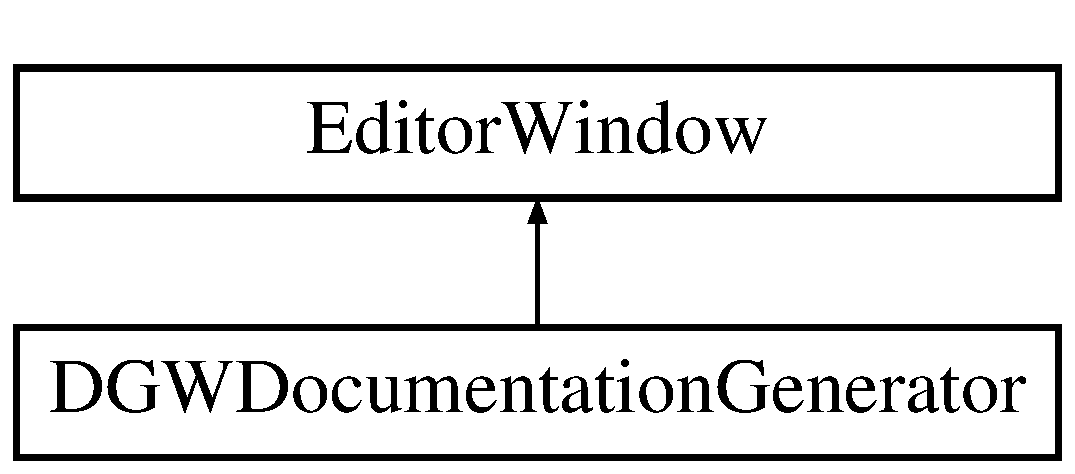
\includegraphics[height=2.000000cm]{d9/dac/classDoxygenGeneratorWindow_1_1DGWDocumentationGenerator}
\end{center}
\end{figure}
\subsection*{Public Member Functions}
\subsection*{Static Public Member Functions}
\subsection*{Data Fields}
\subsection*{Private Member Functions}
\subsection*{Static Private Member Functions}
\subsection*{Private Attributes}
\subsection*{Static Private Attributes}


\subsection{Detailed Description}
D\+GW Documentation generator is a class to generate the documentation by Doxygen automatically 

\subsection{Member Function Documentation}
\mbox{\Hypertarget{classDoxygenGeneratorWindow_1_1DGWDocumentationGenerator_af4de68005ecebdd50b0a3a95b771a2da}\label{classDoxygenGeneratorWindow_1_1DGWDocumentationGenerator_af4de68005ecebdd50b0a3a95b771a2da}} 
\index{Doxygen\+Generator\+Window\+::\+D\+G\+W\+Documentation\+Generator@{Doxygen\+Generator\+Window\+::\+D\+G\+W\+Documentation\+Generator}!Finish\+Doxygen@{Finish\+Doxygen}}
\index{Finish\+Doxygen@{Finish\+Doxygen}!Doxygen\+Generator\+Window\+::\+D\+G\+W\+Documentation\+Generator@{Doxygen\+Generator\+Window\+::\+D\+G\+W\+Documentation\+Generator}}
\subsubsection{\texorpdfstring{Finish\+Doxygen()}{FinishDoxygen()}}
{\footnotesize\ttfamily void Finish\+Doxygen (\begin{DoxyParamCaption}{ }\end{DoxyParamCaption})\hspace{0.3cm}{\ttfamily [private]}}



Finish generation. 

\mbox{\Hypertarget{classDoxygenGeneratorWindow_1_1DGWDocumentationGenerator_a8c1de1d8e5dfe78335d819c5adfcc5c2}\label{classDoxygenGeneratorWindow_1_1DGWDocumentationGenerator_a8c1de1d8e5dfe78335d819c5adfcc5c2}} 
\index{Doxygen\+Generator\+Window\+::\+D\+G\+W\+Documentation\+Generator@{Doxygen\+Generator\+Window\+::\+D\+G\+W\+Documentation\+Generator}!Load\+Preferences@{Load\+Preferences}}
\index{Load\+Preferences@{Load\+Preferences}!Doxygen\+Generator\+Window\+::\+D\+G\+W\+Documentation\+Generator@{Doxygen\+Generator\+Window\+::\+D\+G\+W\+Documentation\+Generator}}
\subsubsection{\texorpdfstring{Load\+Preferences()}{LoadPreferences()}}
{\footnotesize\ttfamily void Load\+Preferences (\begin{DoxyParamCaption}{ }\end{DoxyParamCaption})\hspace{0.3cm}{\ttfamily [private]}}



Load the preferences. 

\mbox{\Hypertarget{classDoxygenGeneratorWindow_1_1DGWDocumentationGenerator_ad7d9716d5d31ecea6d54e73c05c1efe4}\label{classDoxygenGeneratorWindow_1_1DGWDocumentationGenerator_ad7d9716d5d31ecea6d54e73c05c1efe4}} 
\index{Doxygen\+Generator\+Window\+::\+D\+G\+W\+Documentation\+Generator@{Doxygen\+Generator\+Window\+::\+D\+G\+W\+Documentation\+Generator}!On\+Enable@{On\+Enable}}
\index{On\+Enable@{On\+Enable}!Doxygen\+Generator\+Window\+::\+D\+G\+W\+Documentation\+Generator@{Doxygen\+Generator\+Window\+::\+D\+G\+W\+Documentation\+Generator}}
\subsubsection{\texorpdfstring{On\+Enable()}{OnEnable()}}
{\footnotesize\ttfamily void On\+Enable (\begin{DoxyParamCaption}{ }\end{DoxyParamCaption})}



Raises the enable event. 

\mbox{\Hypertarget{classDoxygenGeneratorWindow_1_1DGWDocumentationGenerator_a452f9d1dabef6a4d443f80af717a60eb}\label{classDoxygenGeneratorWindow_1_1DGWDocumentationGenerator_a452f9d1dabef6a4d443f80af717a60eb}} 
\index{Doxygen\+Generator\+Window\+::\+D\+G\+W\+Documentation\+Generator@{Doxygen\+Generator\+Window\+::\+D\+G\+W\+Documentation\+Generator}!On\+G\+UI@{On\+G\+UI}}
\index{On\+G\+UI@{On\+G\+UI}!Doxygen\+Generator\+Window\+::\+D\+G\+W\+Documentation\+Generator@{Doxygen\+Generator\+Window\+::\+D\+G\+W\+Documentation\+Generator}}
\subsubsection{\texorpdfstring{On\+G\+U\+I()}{OnGUI()}}
{\footnotesize\ttfamily void On\+G\+UI (\begin{DoxyParamCaption}{ }\end{DoxyParamCaption})\hspace{0.3cm}{\ttfamily [private]}}



Raises the G\+UI event. 

\mbox{\Hypertarget{classDoxygenGeneratorWindow_1_1DGWDocumentationGenerator_aa35c9b342138fb62fd6e5cb5f1b8082c}\label{classDoxygenGeneratorWindow_1_1DGWDocumentationGenerator_aa35c9b342138fb62fd6e5cb5f1b8082c}} 
\index{Doxygen\+Generator\+Window\+::\+D\+G\+W\+Documentation\+Generator@{Doxygen\+Generator\+Window\+::\+D\+G\+W\+Documentation\+Generator}!Path\+Config@{Path\+Config}}
\index{Path\+Config@{Path\+Config}!Doxygen\+Generator\+Window\+::\+D\+G\+W\+Documentation\+Generator@{Doxygen\+Generator\+Window\+::\+D\+G\+W\+Documentation\+Generator}}
\subsubsection{\texorpdfstring{Path\+Config()}{PathConfig()}}
{\footnotesize\ttfamily string Path\+Config (\begin{DoxyParamCaption}{ }\end{DoxyParamCaption})\hspace{0.3cm}{\ttfamily [private]}}



Return the path of the config. 

\begin{DoxyReturn}{Returns}
The Path.
\end{DoxyReturn}
\mbox{\Hypertarget{classDoxygenGeneratorWindow_1_1DGWDocumentationGenerator_a66f90d8aa6627d3c58fa37c413821cc7}\label{classDoxygenGeneratorWindow_1_1DGWDocumentationGenerator_a66f90d8aa6627d3c58fa37c413821cc7}} 
\index{Doxygen\+Generator\+Window\+::\+D\+G\+W\+Documentation\+Generator@{Doxygen\+Generator\+Window\+::\+D\+G\+W\+Documentation\+Generator}!Path\+Doxygen\+Config@{Path\+Doxygen\+Config}}
\index{Path\+Doxygen\+Config@{Path\+Doxygen\+Config}!Doxygen\+Generator\+Window\+::\+D\+G\+W\+Documentation\+Generator@{Doxygen\+Generator\+Window\+::\+D\+G\+W\+Documentation\+Generator}}
\subsubsection{\texorpdfstring{Path\+Doxygen\+Config()}{PathDoxygenConfig()}}
{\footnotesize\ttfamily string Path\+Doxygen\+Config (\begin{DoxyParamCaption}{ }\end{DoxyParamCaption})\hspace{0.3cm}{\ttfamily [private]}}



Return the path of doxygen config. 

\begin{DoxyReturn}{Returns}
The doxygen Path.
\end{DoxyReturn}
\mbox{\Hypertarget{classDoxygenGeneratorWindow_1_1DGWDocumentationGenerator_a5bac79a047248fc6d5d4b536c2550ee2}\label{classDoxygenGeneratorWindow_1_1DGWDocumentationGenerator_a5bac79a047248fc6d5d4b536c2550ee2}} 
\index{Doxygen\+Generator\+Window\+::\+D\+G\+W\+Documentation\+Generator@{Doxygen\+Generator\+Window\+::\+D\+G\+W\+Documentation\+Generator}!Prepare\+Window@{Prepare\+Window}}
\index{Prepare\+Window@{Prepare\+Window}!Doxygen\+Generator\+Window\+::\+D\+G\+W\+Documentation\+Generator@{Doxygen\+Generator\+Window\+::\+D\+G\+W\+Documentation\+Generator}}
\subsubsection{\texorpdfstring{Prepare\+Window()}{PrepareWindow()}}
{\footnotesize\ttfamily static void Prepare\+Window (\begin{DoxyParamCaption}{ }\end{DoxyParamCaption})\hspace{0.3cm}{\ttfamily [static]}, {\ttfamily [private]}}



Prepare the window. 

\mbox{\Hypertarget{classDoxygenGeneratorWindow_1_1DGWDocumentationGenerator_a5c3c6b8cf003b0da03afec0541c6ced5}\label{classDoxygenGeneratorWindow_1_1DGWDocumentationGenerator_a5c3c6b8cf003b0da03afec0541c6ced5}} 
\index{Doxygen\+Generator\+Window\+::\+D\+G\+W\+Documentation\+Generator@{Doxygen\+Generator\+Window\+::\+D\+G\+W\+Documentation\+Generator}!Run\+Doxygen@{Run\+Doxygen}}
\index{Run\+Doxygen@{Run\+Doxygen}!Doxygen\+Generator\+Window\+::\+D\+G\+W\+Documentation\+Generator@{Doxygen\+Generator\+Window\+::\+D\+G\+W\+Documentation\+Generator}}
\subsubsection{\texorpdfstring{Run\+Doxygen()}{RunDoxygen()}}
{\footnotesize\ttfamily void Run\+Doxygen (\begin{DoxyParamCaption}{ }\end{DoxyParamCaption})\hspace{0.3cm}{\ttfamily [private]}}



Run doxygen! 

\mbox{\Hypertarget{classDoxygenGeneratorWindow_1_1DGWDocumentationGenerator_ac77ed02a599b36b8bf3779ef68908535}\label{classDoxygenGeneratorWindow_1_1DGWDocumentationGenerator_ac77ed02a599b36b8bf3779ef68908535}} 
\index{Doxygen\+Generator\+Window\+::\+D\+G\+W\+Documentation\+Generator@{Doxygen\+Generator\+Window\+::\+D\+G\+W\+Documentation\+Generator}!Save\+Preferences@{Save\+Preferences}}
\index{Save\+Preferences@{Save\+Preferences}!Doxygen\+Generator\+Window\+::\+D\+G\+W\+Documentation\+Generator@{Doxygen\+Generator\+Window\+::\+D\+G\+W\+Documentation\+Generator}}
\subsubsection{\texorpdfstring{Save\+Preferences()}{SavePreferences()}}
{\footnotesize\ttfamily void Save\+Preferences (\begin{DoxyParamCaption}{ }\end{DoxyParamCaption})\hspace{0.3cm}{\ttfamily [private]}}



Save the preferences. 

\mbox{\Hypertarget{classDoxygenGeneratorWindow_1_1DGWDocumentationGenerator_ae13b9614dce4bcdd3fcc24354910a4a6}\label{classDoxygenGeneratorWindow_1_1DGWDocumentationGenerator_ae13b9614dce4bcdd3fcc24354910a4a6}} 
\index{Doxygen\+Generator\+Window\+::\+D\+G\+W\+Documentation\+Generator@{Doxygen\+Generator\+Window\+::\+D\+G\+W\+Documentation\+Generator}!Shared\+Instance@{Shared\+Instance}}
\index{Shared\+Instance@{Shared\+Instance}!Doxygen\+Generator\+Window\+::\+D\+G\+W\+Documentation\+Generator@{Doxygen\+Generator\+Window\+::\+D\+G\+W\+Documentation\+Generator}}
\subsubsection{\texorpdfstring{Shared\+Instance()}{SharedInstance()}}
{\footnotesize\ttfamily static D\+G\+W\+Documentation\+Generator Shared\+Instance (\begin{DoxyParamCaption}{ }\end{DoxyParamCaption})\hspace{0.3cm}{\ttfamily [static]}}



Ascencor to shared instance. 

\begin{DoxyReturn}{Returns}
The shared instance.
\end{DoxyReturn}
\mbox{\Hypertarget{classDoxygenGeneratorWindow_1_1DGWDocumentationGenerator_a1bf4af51249f8e35e232f40b0b73da17}\label{classDoxygenGeneratorWindow_1_1DGWDocumentationGenerator_a1bf4af51249f8e35e232f40b0b73da17}} 
\index{Doxygen\+Generator\+Window\+::\+D\+G\+W\+Documentation\+Generator@{Doxygen\+Generator\+Window\+::\+D\+G\+W\+Documentation\+Generator}!Yes\+Or\+No@{Yes\+Or\+No}}
\index{Yes\+Or\+No@{Yes\+Or\+No}!Doxygen\+Generator\+Window\+::\+D\+G\+W\+Documentation\+Generator@{Doxygen\+Generator\+Window\+::\+D\+G\+W\+Documentation\+Generator}}
\subsubsection{\texorpdfstring{Yes\+Or\+No()}{YesOrNo()}}
{\footnotesize\ttfamily string Yes\+Or\+No (\begin{DoxyParamCaption}\item[{bool}]{s\+Value }\end{DoxyParamCaption})}



Conversion bool to string Y\+ES or NO for config fill. 

\begin{DoxyReturn}{Returns}
The or no.
\end{DoxyReturn}

\begin{DoxyParams}{Parameters}
{\em s\+Value} & If set to {\ttfamily true} value.\\
\hline
\end{DoxyParams}


\subsection{Field Documentation}
\mbox{\Hypertarget{classDoxygenGeneratorWindow_1_1DGWDocumentationGenerator_a3ac8443104c638c0b61a841fec5361b4}\label{classDoxygenGeneratorWindow_1_1DGWDocumentationGenerator_a3ac8443104c638c0b61a841fec5361b4}} 
\index{Doxygen\+Generator\+Window\+::\+D\+G\+W\+Documentation\+Generator@{Doxygen\+Generator\+Window\+::\+D\+G\+W\+Documentation\+Generator}!Config@{Config}}
\index{Config@{Config}!Doxygen\+Generator\+Window\+::\+D\+G\+W\+Documentation\+Generator@{Doxygen\+Generator\+Window\+::\+D\+G\+W\+Documentation\+Generator}}
\subsubsection{\texorpdfstring{Config}{Config}}
{\footnotesize\ttfamily D\+G\+W\+Config Config}



The config of this project. 

\mbox{\Hypertarget{classDoxygenGeneratorWindow_1_1DGWDocumentationGenerator_a52d47c7d99e5e807edb0fd97e83b1939}\label{classDoxygenGeneratorWindow_1_1DGWDocumentationGenerator_a52d47c7d99e5e807edb0fd97e83b1939}} 
\index{Doxygen\+Generator\+Window\+::\+D\+G\+W\+Documentation\+Generator@{Doxygen\+Generator\+Window\+::\+D\+G\+W\+Documentation\+Generator}!K\+\_\+\+U\+R\+L\+\_\+\+D\+O\+X\+Y\+G\+EN@{K\+\_\+\+U\+R\+L\+\_\+\+D\+O\+X\+Y\+G\+EN}}
\index{K\+\_\+\+U\+R\+L\+\_\+\+D\+O\+X\+Y\+G\+EN@{K\+\_\+\+U\+R\+L\+\_\+\+D\+O\+X\+Y\+G\+EN}!Doxygen\+Generator\+Window\+::\+D\+G\+W\+Documentation\+Generator@{Doxygen\+Generator\+Window\+::\+D\+G\+W\+Documentation\+Generator}}
\subsubsection{\texorpdfstring{K\+\_\+\+U\+R\+L\+\_\+\+D\+O\+X\+Y\+G\+EN}{K\_URL\_DOXYGEN}}
{\footnotesize\ttfamily const string K\+\_\+\+U\+R\+L\+\_\+\+D\+O\+X\+Y\+G\+EN = \char`\"{}http\+://www.\+stack.\+nl/$\sim$dimitri/doxygen/download.\+html\char`\"{}}



The D\+O\+X\+Y\+G\+EN U\+RL. 

\mbox{\Hypertarget{classDoxygenGeneratorWindow_1_1DGWDocumentationGenerator_aac78f64d10530e9c66b36a80b0804e3c}\label{classDoxygenGeneratorWindow_1_1DGWDocumentationGenerator_aac78f64d10530e9c66b36a80b0804e3c}} 
\index{Doxygen\+Generator\+Window\+::\+D\+G\+W\+Documentation\+Generator@{Doxygen\+Generator\+Window\+::\+D\+G\+W\+Documentation\+Generator}!k\+Group\+Reset\+State@{k\+Group\+Reset\+State}}
\index{k\+Group\+Reset\+State@{k\+Group\+Reset\+State}!Doxygen\+Generator\+Window\+::\+D\+G\+W\+Documentation\+Generator@{Doxygen\+Generator\+Window\+::\+D\+G\+W\+Documentation\+Generator}}
\subsubsection{\texorpdfstring{k\+Group\+Reset\+State}{kGroupResetState}}
{\footnotesize\ttfamily bool k\+Group\+Reset\+State = false\hspace{0.3cm}{\ttfamily [static]}, {\ttfamily [private]}}



The state of the group reset. 

\mbox{\Hypertarget{classDoxygenGeneratorWindow_1_1DGWDocumentationGenerator_a0c5205fb7226436a3bd68a6ca750ee45}\label{classDoxygenGeneratorWindow_1_1DGWDocumentationGenerator_a0c5205fb7226436a3bd68a6ca750ee45}} 
\index{Doxygen\+Generator\+Window\+::\+D\+G\+W\+Documentation\+Generator@{Doxygen\+Generator\+Window\+::\+D\+G\+W\+Documentation\+Generator}!k\+Shared\+Instance@{k\+Shared\+Instance}}
\index{k\+Shared\+Instance@{k\+Shared\+Instance}!Doxygen\+Generator\+Window\+::\+D\+G\+W\+Documentation\+Generator@{Doxygen\+Generator\+Window\+::\+D\+G\+W\+Documentation\+Generator}}
\subsubsection{\texorpdfstring{k\+Shared\+Instance}{kSharedInstance}}
{\footnotesize\ttfamily D\+G\+W\+Documentation\+Generator k\+Shared\+Instance\hspace{0.3cm}{\ttfamily [static]}, {\ttfamily [private]}}



The shared instance. 

\mbox{\Hypertarget{classDoxygenGeneratorWindow_1_1DGWDocumentationGenerator_ab18fc7369e955cd707822f599cd2a726}\label{classDoxygenGeneratorWindow_1_1DGWDocumentationGenerator_ab18fc7369e955cd707822f599cd2a726}} 
\index{Doxygen\+Generator\+Window\+::\+D\+G\+W\+Documentation\+Generator@{Doxygen\+Generator\+Window\+::\+D\+G\+W\+Documentation\+Generator}!Scroll\+Position@{Scroll\+Position}}
\index{Scroll\+Position@{Scroll\+Position}!Doxygen\+Generator\+Window\+::\+D\+G\+W\+Documentation\+Generator@{Doxygen\+Generator\+Window\+::\+D\+G\+W\+Documentation\+Generator}}
\subsubsection{\texorpdfstring{Scroll\+Position}{ScrollPosition}}
{\footnotesize\ttfamily Vector2 Scroll\+Position\hspace{0.3cm}{\ttfamily [private]}}



The scroll position of scrollview. 

\mbox{\Hypertarget{classDoxygenGeneratorWindow_1_1DGWDocumentationGenerator_a081bcc409dad2dc380fa85c9e1c3235d}\label{classDoxygenGeneratorWindow_1_1DGWDocumentationGenerator_a081bcc409dad2dc380fa85c9e1c3235d}} 
\index{Doxygen\+Generator\+Window\+::\+D\+G\+W\+Documentation\+Generator@{Doxygen\+Generator\+Window\+::\+D\+G\+W\+Documentation\+Generator}!Work\+In\+Progress@{Work\+In\+Progress}}
\index{Work\+In\+Progress@{Work\+In\+Progress}!Doxygen\+Generator\+Window\+::\+D\+G\+W\+Documentation\+Generator@{Doxygen\+Generator\+Window\+::\+D\+G\+W\+Documentation\+Generator}}
\subsubsection{\texorpdfstring{Work\+In\+Progress}{WorkInProgress}}
{\footnotesize\ttfamily bool Work\+In\+Progress = false}



Work in progress or not. 



The documentation for this class was generated from the following file\+:\begin{DoxyCompactItemize}
\item 
Assets/\+Doxygen\+Generator\+Window/\+Editor/\+D\+G\+W\+Documentation\+Generator/\hyperlink{DGWDocumentationGenerator_8cs}{D\+G\+W\+Documentation\+Generator.\+cs}\end{DoxyCompactItemize}

\hypertarget{classDoxygenGeneratorWindow_1_1DGWEditorMenu}{}\section{D\+G\+W\+Editor\+Menu Class Reference}
\label{classDoxygenGeneratorWindow_1_1DGWEditorMenu}\index{D\+G\+W\+Editor\+Menu@{D\+G\+W\+Editor\+Menu}}


D\+GW editor menu.  


\subsection*{Public Member Functions}


\subsection{Detailed Description}
D\+GW editor menu. 



\subsection{Constructor \& Destructor Documentation}
\mbox{\Hypertarget{classDoxygenGeneratorWindow_1_1DGWEditorMenu_abc03c777b285ed315fc74db7340b3664}\label{classDoxygenGeneratorWindow_1_1DGWEditorMenu_abc03c777b285ed315fc74db7340b3664}} 
\index{Doxygen\+Generator\+Window\+::\+D\+G\+W\+Editor\+Menu@{Doxygen\+Generator\+Window\+::\+D\+G\+W\+Editor\+Menu}!D\+G\+W\+Editor\+Menu@{D\+G\+W\+Editor\+Menu}}
\index{D\+G\+W\+Editor\+Menu@{D\+G\+W\+Editor\+Menu}!Doxygen\+Generator\+Window\+::\+D\+G\+W\+Editor\+Menu@{Doxygen\+Generator\+Window\+::\+D\+G\+W\+Editor\+Menu}}
\subsubsection{\texorpdfstring{D\+G\+W\+Editor\+Menu()}{DGWEditorMenu()}}
{\footnotesize\ttfamily D\+G\+W\+Editor\+Menu (\begin{DoxyParamCaption}{ }\end{DoxyParamCaption})}



Initializes a new instance of the \hyperlink{classDoxygenGeneratorWindow_1_1DGWEditorMenu}{Doxygen\+Generator\+Window.\+D\+G\+W\+Editor\+Menu} class. 



The documentation for this class was generated from the following file\+:\begin{DoxyCompactItemize}
\item 
Assets/\+Doxygen\+Generator\+Window/\+Editor/\+D\+G\+W\+Editor\+Menu/\hyperlink{DGWEditorMenu_8cs}{D\+G\+W\+Editor\+Menu.\+cs}\end{DoxyCompactItemize}

\hypertarget{classDoxygenGeneratorWindow_1_1DGWFindPackage}{}\section{D\+G\+W\+Find\+Package Class Reference}
\label{classDoxygenGeneratorWindow_1_1DGWFindPackage}\index{D\+G\+W\+Find\+Package@{D\+G\+W\+Find\+Package}}


Find package path class. Use the Scriptable\+Object to find the path of this package  


Inheritance diagram for D\+G\+W\+Find\+Package\+:\begin{figure}[H]
\begin{center}
\leavevmode
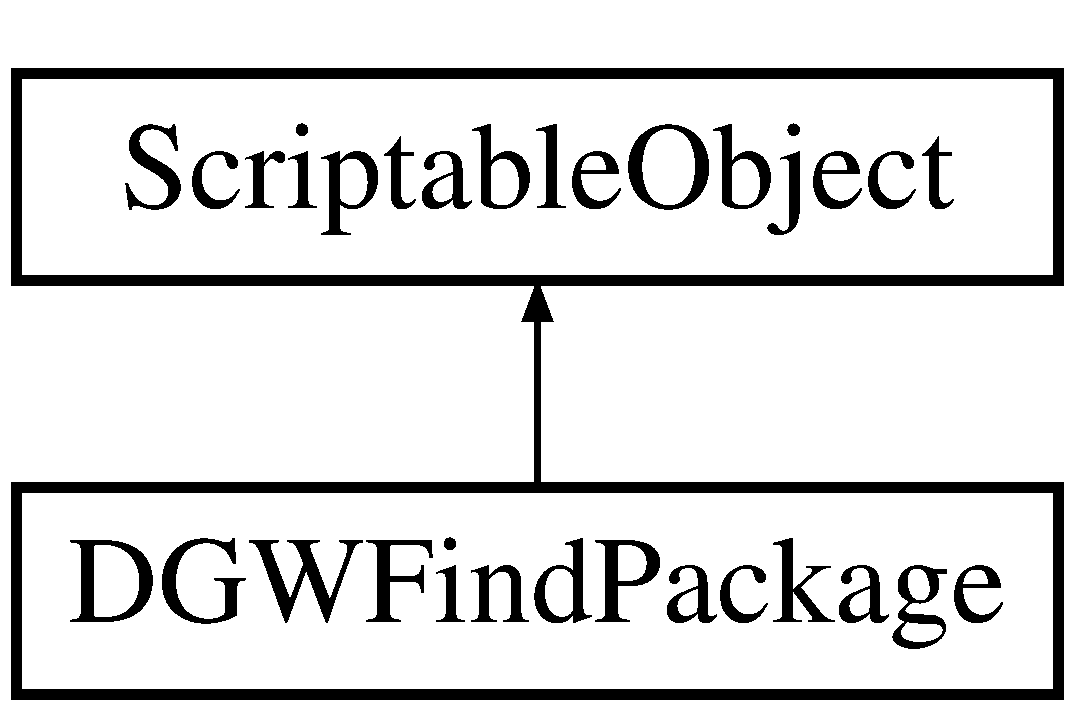
\includegraphics[height=2.000000cm]{d3/d50/classDoxygenGeneratorWindow_1_1DGWFindPackage}
\end{center}
\end{figure}
\subsection*{Public Member Functions}
\subsection*{Static Public Member Functions}
\subsection*{Data Fields}
\subsection*{Static Private Attributes}


\subsection{Detailed Description}
Find package path class. Use the Scriptable\+Object to find the path of this package 



\subsection{Member Function Documentation}
\mbox{\Hypertarget{classDoxygenGeneratorWindow_1_1DGWFindPackage_a419068e8651e24c994cf1d34b24dd4b0}\label{classDoxygenGeneratorWindow_1_1DGWFindPackage_a419068e8651e24c994cf1d34b24dd4b0}} 
\index{Doxygen\+Generator\+Window\+::\+D\+G\+W\+Find\+Package@{Doxygen\+Generator\+Window\+::\+D\+G\+W\+Find\+Package}!Path\+Of\+Package@{Path\+Of\+Package}}
\index{Path\+Of\+Package@{Path\+Of\+Package}!Doxygen\+Generator\+Window\+::\+D\+G\+W\+Find\+Package@{Doxygen\+Generator\+Window\+::\+D\+G\+W\+Find\+Package}}
\subsubsection{\texorpdfstring{Path\+Of\+Package()}{PathOfPackage()}}
{\footnotesize\ttfamily static string Path\+Of\+Package (\begin{DoxyParamCaption}\item[{string}]{s\+Add\+Path = {\ttfamily \char`\"{}\char`\"{}} }\end{DoxyParamCaption})\hspace{0.3cm}{\ttfamily [static]}}



Packages the path. 

\begin{DoxyReturn}{Returns}
The path.
\end{DoxyReturn}

\begin{DoxyParams}{Parameters}
{\em s\+Add\+Path} & add path.\\
\hline
\end{DoxyParams}
\mbox{\Hypertarget{classDoxygenGeneratorWindow_1_1DGWFindPackage_a5f43d04fc81cb9065084c01b5d2c3b01}\label{classDoxygenGeneratorWindow_1_1DGWFindPackage_a5f43d04fc81cb9065084c01b5d2c3b01}} 
\index{Doxygen\+Generator\+Window\+::\+D\+G\+W\+Find\+Package@{Doxygen\+Generator\+Window\+::\+D\+G\+W\+Find\+Package}!Read\+Paths@{Read\+Paths}}
\index{Read\+Paths@{Read\+Paths}!Doxygen\+Generator\+Window\+::\+D\+G\+W\+Find\+Package@{Doxygen\+Generator\+Window\+::\+D\+G\+W\+Find\+Package}}
\subsubsection{\texorpdfstring{Read\+Paths()}{ReadPaths()}}
{\footnotesize\ttfamily void Read\+Paths (\begin{DoxyParamCaption}{ }\end{DoxyParamCaption})}



Reads the paths. 

\mbox{\Hypertarget{classDoxygenGeneratorWindow_1_1DGWFindPackage_ab232fc3aceaf32c98c4febb05da8b8b7}\label{classDoxygenGeneratorWindow_1_1DGWFindPackage_ab232fc3aceaf32c98c4febb05da8b8b7}} 
\index{Doxygen\+Generator\+Window\+::\+D\+G\+W\+Find\+Package@{Doxygen\+Generator\+Window\+::\+D\+G\+W\+Find\+Package}!Shared\+Instance@{Shared\+Instance}}
\index{Shared\+Instance@{Shared\+Instance}!Doxygen\+Generator\+Window\+::\+D\+G\+W\+Find\+Package@{Doxygen\+Generator\+Window\+::\+D\+G\+W\+Find\+Package}}
\subsubsection{\texorpdfstring{Shared\+Instance()}{SharedInstance()}}
{\footnotesize\ttfamily static D\+G\+W\+Find\+Package Shared\+Instance (\begin{DoxyParamCaption}{ }\end{DoxyParamCaption})\hspace{0.3cm}{\ttfamily [static]}}



Ascencor to shared instance. 

\begin{DoxyReturn}{Returns}
The shared instance.
\end{DoxyReturn}


\subsection{Field Documentation}
\mbox{\Hypertarget{classDoxygenGeneratorWindow_1_1DGWFindPackage_aec97c04918bf99ba1a2cbc0f8cd4f4e3}\label{classDoxygenGeneratorWindow_1_1DGWFindPackage_aec97c04918bf99ba1a2cbc0f8cd4f4e3}} 
\index{Doxygen\+Generator\+Window\+::\+D\+G\+W\+Find\+Package@{Doxygen\+Generator\+Window\+::\+D\+G\+W\+Find\+Package}!k\+Shared\+Instance@{k\+Shared\+Instance}}
\index{k\+Shared\+Instance@{k\+Shared\+Instance}!Doxygen\+Generator\+Window\+::\+D\+G\+W\+Find\+Package@{Doxygen\+Generator\+Window\+::\+D\+G\+W\+Find\+Package}}
\subsubsection{\texorpdfstring{k\+Shared\+Instance}{kSharedInstance}}
{\footnotesize\ttfamily D\+G\+W\+Find\+Package k\+Shared\+Instance\hspace{0.3cm}{\ttfamily [static]}, {\ttfamily [private]}}



The shared instance. 

\mbox{\Hypertarget{classDoxygenGeneratorWindow_1_1DGWFindPackage_a0f4063fb020b7475f93d486db091c472}\label{classDoxygenGeneratorWindow_1_1DGWFindPackage_a0f4063fb020b7475f93d486db091c472}} 
\index{Doxygen\+Generator\+Window\+::\+D\+G\+W\+Find\+Package@{Doxygen\+Generator\+Window\+::\+D\+G\+W\+Find\+Package}!Script\+File\+Path@{Script\+File\+Path}}
\index{Script\+File\+Path@{Script\+File\+Path}!Doxygen\+Generator\+Window\+::\+D\+G\+W\+Find\+Package@{Doxygen\+Generator\+Window\+::\+D\+G\+W\+Find\+Package}}
\subsubsection{\texorpdfstring{Script\+File\+Path}{ScriptFilePath}}
{\footnotesize\ttfamily string Script\+File\+Path}



The script file path. 

\mbox{\Hypertarget{classDoxygenGeneratorWindow_1_1DGWFindPackage_a2e18e42277429a27bab9ae2b0f852b7b}\label{classDoxygenGeneratorWindow_1_1DGWFindPackage_a2e18e42277429a27bab9ae2b0f852b7b}} 
\index{Doxygen\+Generator\+Window\+::\+D\+G\+W\+Find\+Package@{Doxygen\+Generator\+Window\+::\+D\+G\+W\+Find\+Package}!Script\+Folder@{Script\+Folder}}
\index{Script\+Folder@{Script\+Folder}!Doxygen\+Generator\+Window\+::\+D\+G\+W\+Find\+Package@{Doxygen\+Generator\+Window\+::\+D\+G\+W\+Find\+Package}}
\subsubsection{\texorpdfstring{Script\+Folder}{ScriptFolder}}
{\footnotesize\ttfamily string Script\+Folder}



The script folder. 

\mbox{\Hypertarget{classDoxygenGeneratorWindow_1_1DGWFindPackage_a89e7ed4aa9d4cda9731cd6b1fd8ce5c8}\label{classDoxygenGeneratorWindow_1_1DGWFindPackage_a89e7ed4aa9d4cda9731cd6b1fd8ce5c8}} 
\index{Doxygen\+Generator\+Window\+::\+D\+G\+W\+Find\+Package@{Doxygen\+Generator\+Window\+::\+D\+G\+W\+Find\+Package}!Script\+Folder\+From\+Assets@{Script\+Folder\+From\+Assets}}
\index{Script\+Folder\+From\+Assets@{Script\+Folder\+From\+Assets}!Doxygen\+Generator\+Window\+::\+D\+G\+W\+Find\+Package@{Doxygen\+Generator\+Window\+::\+D\+G\+W\+Find\+Package}}
\subsubsection{\texorpdfstring{Script\+Folder\+From\+Assets}{ScriptFolderFromAssets}}
{\footnotesize\ttfamily string Script\+Folder\+From\+Assets}



The script folder from assets. 



The documentation for this class was generated from the following file\+:\begin{DoxyCompactItemize}
\item 
Assets/\+Doxygen\+Generator\+Window/\hyperlink{DGWFindPackage_8cs}{D\+G\+W\+Find\+Package.\+cs}\end{DoxyCompactItemize}

\hypertarget{classDoxygenGeneratorWindow_1_1DGWMacroDefine}{}\doxysection{D\+G\+W\+Macro\+Define Class Reference}
\label{classDoxygenGeneratorWindow_1_1DGWMacroDefine}\index{DGWMacroDefine@{DGWMacroDefine}}


Macro define can find if k\+Macro is set in the settings and add it if necessary. This class auto run at build project. You can use k\+Macro in precompile definition.  


Inheritance diagram for D\+G\+W\+Macro\+Define\+:\begin{figure}[H]
\begin{center}
\leavevmode
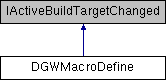
\includegraphics[height=2.000000cm]{classDoxygenGeneratorWindow_1_1DGWMacroDefine}
\end{center}
\end{figure}
\doxysubsection*{Public Member Functions}
\doxysubsection*{Properties}
\doxysubsection*{Static Private Member Functions}
\doxysubsection*{Static Private Attributes}


\doxysubsection{Detailed Description}
Macro define can find if k\+Macro is set in the settings and add it if necessary. This class auto run at build project. You can use k\+Macro in precompile definition. 



\doxysubsection{Constructor \& Destructor Documentation}
\mbox{\Hypertarget{classDoxygenGeneratorWindow_1_1DGWMacroDefine_a6cb0c63ccea4107b1946288c5f69a96f}\label{classDoxygenGeneratorWindow_1_1DGWMacroDefine_a6cb0c63ccea4107b1946288c5f69a96f}} 
\index{DGWMacroDefine@{DGWMacroDefine}!DGWMacroDefine@{DGWMacroDefine}}
\index{DGWMacroDefine@{DGWMacroDefine}!DGWMacroDefine@{DGWMacroDefine}}
\doxysubsubsection{\texorpdfstring{DGWMacroDefine()}{DGWMacroDefine()}}
{\footnotesize\ttfamily static D\+G\+W\+Macro\+Define (\begin{DoxyParamCaption}{ }\end{DoxyParamCaption})\hspace{0.3cm}{\ttfamily [static]}, {\ttfamily [private]}}



Initializes the \mbox{\hyperlink{classDoxygenGeneratorWindow_1_1DGWMacroDefine}{D\+G\+W\+Macro\+Define}} class. Instance k\+Shared\+Instance to use it when method On\+Active\+Build\+Target\+Changed must be invoked 



\doxysubsection{Member Function Documentation}
\mbox{\Hypertarget{classDoxygenGeneratorWindow_1_1DGWMacroDefine_a90757509429b8c1c3a47f368d16a0aa8}\label{classDoxygenGeneratorWindow_1_1DGWMacroDefine_a90757509429b8c1c3a47f368d16a0aa8}} 
\index{DGWMacroDefine@{DGWMacroDefine}!InstallMacro@{InstallMacro}}
\index{InstallMacro@{InstallMacro}!DGWMacroDefine@{DGWMacroDefine}}
\doxysubsubsection{\texorpdfstring{InstallMacro()}{InstallMacro()}}
{\footnotesize\ttfamily void Install\+Macro (\begin{DoxyParamCaption}\item[{Build\+Target\+Group}]{s\+Build\+Target }\end{DoxyParamCaption})}



Installs the macro. 


\begin{DoxyParams}{Parameters}
{\em s\+Build\+Target} & S build target.\\
\hline
\end{DoxyParams}
\mbox{\Hypertarget{classDoxygenGeneratorWindow_1_1DGWMacroDefine_aa57b1e003d8b9f783b6815e2e5969018}\label{classDoxygenGeneratorWindow_1_1DGWMacroDefine_aa57b1e003d8b9f783b6815e2e5969018}} 
\index{DGWMacroDefine@{DGWMacroDefine}!InstallMacroAll@{InstallMacroAll}}
\index{InstallMacroAll@{InstallMacroAll}!DGWMacroDefine@{DGWMacroDefine}}
\doxysubsubsection{\texorpdfstring{InstallMacroAll()}{InstallMacroAll()}}
{\footnotesize\ttfamily void Install\+Macro\+All (\begin{DoxyParamCaption}{ }\end{DoxyParamCaption})}



Installs the macro in all build target. 

\mbox{\Hypertarget{classDoxygenGeneratorWindow_1_1DGWMacroDefine_a462eaf2e8a4b1c90f3b7551d2b28fefb}\label{classDoxygenGeneratorWindow_1_1DGWMacroDefine_a462eaf2e8a4b1c90f3b7551d2b28fefb}} 
\index{DGWMacroDefine@{DGWMacroDefine}!OnActiveBuildTargetChanged@{OnActiveBuildTargetChanged}}
\index{OnActiveBuildTargetChanged@{OnActiveBuildTargetChanged}!DGWMacroDefine@{DGWMacroDefine}}
\doxysubsubsection{\texorpdfstring{OnActiveBuildTargetChanged()}{OnActiveBuildTargetChanged()}}
{\footnotesize\ttfamily void On\+Active\+Build\+Target\+Changed (\begin{DoxyParamCaption}\item[{Build\+Target}]{previous\+Target,  }\item[{Build\+Target}]{new\+Target }\end{DoxyParamCaption})}



Raises the active build target changed event. 


\begin{DoxyParams}{Parameters}
{\em previous\+Target} & Previous target.\\
\hline
{\em new\+Target} & New target.\\
\hline
\end{DoxyParams}
\mbox{\Hypertarget{classDoxygenGeneratorWindow_1_1DGWMacroDefine_a9ba815b8a4ff2feefdc0e3a7edec07db}\label{classDoxygenGeneratorWindow_1_1DGWMacroDefine_a9ba815b8a4ff2feefdc0e3a7edec07db}} 
\index{DGWMacroDefine@{DGWMacroDefine}!OnChangedPlatform@{OnChangedPlatform}}
\index{OnChangedPlatform@{OnChangedPlatform}!DGWMacroDefine@{DGWMacroDefine}}
\doxysubsubsection{\texorpdfstring{OnChangedPlatform()}{OnChangedPlatform()}}
{\footnotesize\ttfamily void On\+Changed\+Platform (\begin{DoxyParamCaption}{ }\end{DoxyParamCaption})}



Raises the changed platform event. 



\doxysubsection{Field Documentation}
\mbox{\Hypertarget{classDoxygenGeneratorWindow_1_1DGWMacroDefine_acde3a392788fb5e01946c5ca6c2dde3c}\label{classDoxygenGeneratorWindow_1_1DGWMacroDefine_acde3a392788fb5e01946c5ca6c2dde3c}} 
\index{DGWMacroDefine@{DGWMacroDefine}!kMacro@{kMacro}}
\index{kMacro@{kMacro}!DGWMacroDefine@{DGWMacroDefine}}
\doxysubsubsection{\texorpdfstring{kMacro}{kMacro}}
{\footnotesize\ttfamily const string k\+Macro = \char`\"{}D\+O\+X\+Y\+G\+E\+N\+\_\+\+G\+E\+N\+E\+R\+A\+T\+O\+R\+\_\+\+W\+I\+N\+D\+OW\char`\"{}\hspace{0.3cm}{\ttfamily [static]}, {\ttfamily [private]}}



The macro to check in this project. It\textquotesingle{}s tag in settings. The you can use \#if define xxxxx \#endif in your code. 

\mbox{\Hypertarget{classDoxygenGeneratorWindow_1_1DGWMacroDefine_a0cb135a82751baf9f7f44bfb9f70db77}\label{classDoxygenGeneratorWindow_1_1DGWMacroDefine_a0cb135a82751baf9f7f44bfb9f70db77}} 
\index{DGWMacroDefine@{DGWMacroDefine}!kSharedInstance@{kSharedInstance}}
\index{kSharedInstance@{kSharedInstance}!DGWMacroDefine@{DGWMacroDefine}}
\doxysubsubsection{\texorpdfstring{kSharedInstance}{kSharedInstance}}
{\footnotesize\ttfamily \mbox{\hyperlink{classDoxygenGeneratorWindow_1_1DGWMacroDefine_a6cb0c63ccea4107b1946288c5f69a96f}{D\+G\+W\+Macro\+Define}} k\+Shared\+Instance\hspace{0.3cm}{\ttfamily [static]}, {\ttfamily [private]}}



The shared instance used for this class. 



\doxysubsection{Property Documentation}
\mbox{\Hypertarget{classDoxygenGeneratorWindow_1_1DGWMacroDefine_a365dacd9a6045034e8d550713003e2af}\label{classDoxygenGeneratorWindow_1_1DGWMacroDefine_a365dacd9a6045034e8d550713003e2af}} 
\index{DGWMacroDefine@{DGWMacroDefine}!callbackOrder@{callbackOrder}}
\index{callbackOrder@{callbackOrder}!DGWMacroDefine@{DGWMacroDefine}}
\doxysubsubsection{\texorpdfstring{callbackOrder}{callbackOrder}}
{\footnotesize\ttfamily int callback\+Order\hspace{0.3cm}{\ttfamily [get]}}



Gets the callback order for I\+Active\+Build\+Target\+Changed 

The callback order.

The documentation for this class was generated from the following file\+:\begin{DoxyCompactItemize}
\item 
Assets/\+Doxygen\+Generator\+Window/\mbox{\hyperlink{DGWMacroDefine_8cs}{D\+G\+W\+Macro\+Define.\+cs}}\end{DoxyCompactItemize}

\chapter{File Documentation}
\hypertarget{DGWFindPackage_8cs}{}\doxysection{Assets/\+Doxygen\+Generator\+Window/\+D\+G\+W\+Find\+Package.cs File Reference}
\label{DGWFindPackage_8cs}\index{Assets/DoxygenGeneratorWindow/DGWFindPackage.cs@{Assets/DoxygenGeneratorWindow/DGWFindPackage.cs}}
\doxysubsection*{Data Structures}
\begin{DoxyCompactItemize}
\item 
class \mbox{\hyperlink{classDoxygenGeneratorWindow_1_1DGWFindPackage}{D\+G\+W\+Find\+Package}}
\begin{DoxyCompactList}\small\item\em Find package path class. Use the Scriptable\+Object to find the path of this package \end{DoxyCompactList}\end{DoxyCompactItemize}

\hypertarget{DGWMacroDefine_8cs}{}\section{Assets/\+Doxygen\+Generator\+Window/\+D\+G\+W\+Macro\+Define.cs File Reference}
\label{DGWMacroDefine_8cs}\index{Assets/\+Doxygen\+Generator\+Window/\+D\+G\+W\+Macro\+Define.\+cs@{Assets/\+Doxygen\+Generator\+Window/\+D\+G\+W\+Macro\+Define.\+cs}}
\subsection*{Data Structures}
\begin{DoxyCompactItemize}
\item 
class \hyperlink{classDoxygenGeneratorWindow_1_1DGWMacroDefine}{D\+G\+W\+Macro\+Define}
\begin{DoxyCompactList}\small\item\em Macro define can find if k\+Macro is set in the settings and add it if necessary. This class auto run at build project. You can use k\+Macro in precompile definition. \end{DoxyCompactList}\end{DoxyCompactItemize}

\hypertarget{DGWConfig_8cs}{}\doxysection{Assets/\+Doxygen\+Generator\+Window/\+Scripts/\+Editor/\+D\+G\+W\+Config.cs File Reference}
\label{DGWConfig_8cs}\index{Assets/DoxygenGeneratorWindow/Scripts/Editor/DGWConfig.cs@{Assets/DoxygenGeneratorWindow/Scripts/Editor/DGWConfig.cs}}
\doxysubsection*{Data Structures}
\begin{DoxyCompactItemize}
\item 
class \mbox{\hyperlink{classDoxygenGeneratorWindow_1_1DGWConfig}{D\+G\+W\+Config}}
\begin{DoxyCompactList}\small\item\em D\+GW config reccord your config... it\textquotesingle{}s enough! \end{DoxyCompactList}\end{DoxyCompactItemize}

\hypertarget{DGWConstants_8cs}{}\doxysection{Assets/\+Doxygen\+Generator\+Window/\+Scripts/\+Editor/\+D\+G\+W\+Constants.cs File Reference}
\label{DGWConstants_8cs}\index{Assets/DoxygenGeneratorWindow/Scripts/Editor/DGWConstants.cs@{Assets/DoxygenGeneratorWindow/Scripts/Editor/DGWConstants.cs}}
\doxysubsection*{Data Structures}
\begin{DoxyCompactItemize}
\item 
class \mbox{\hyperlink{classDoxygenGeneratorWindow_1_1DGWConstants}{D\+G\+W\+Constants}}
\end{DoxyCompactItemize}

\hypertarget{DGWDocumentationGenerator_8cs}{}\section{Assets/\+Doxygen\+Generator\+Window/\+Editor/\+D\+G\+W\+Documentation\+Generator/\+D\+G\+W\+Documentation\+Generator.cs File Reference}
\label{DGWDocumentationGenerator_8cs}\index{Assets/\+Doxygen\+Generator\+Window/\+Editor/\+D\+G\+W\+Documentation\+Generator/\+D\+G\+W\+Documentation\+Generator.\+cs@{Assets/\+Doxygen\+Generator\+Window/\+Editor/\+D\+G\+W\+Documentation\+Generator/\+D\+G\+W\+Documentation\+Generator.\+cs}}
\subsection*{Data Structures}
\begin{DoxyCompactItemize}
\item 
class \hyperlink{classDoxygenGeneratorWindow_1_1DGWDocumentationGenerator}{D\+G\+W\+Documentation\+Generator}
\begin{DoxyCompactList}\small\item\em D\+GW Documentation generator is a class to generate the documentation by Doxygen automatically \end{DoxyCompactList}\end{DoxyCompactItemize}

\hypertarget{DGWEditorMenu_8cs}{}\doxysection{Assets/\+Doxygen\+Generator\+Window/\+Scripts/\+Editor/\+D\+G\+W\+Editor\+Menu.cs File Reference}
\label{DGWEditorMenu_8cs}\index{Assets/DoxygenGeneratorWindow/Scripts/Editor/DGWEditorMenu.cs@{Assets/DoxygenGeneratorWindow/Scripts/Editor/DGWEditorMenu.cs}}
\doxysubsection*{Data Structures}
\begin{DoxyCompactItemize}
\item 
class \mbox{\hyperlink{classDoxygenGeneratorWindow_1_1DGWEditorMenu}{D\+G\+W\+Editor\+Menu}}
\begin{DoxyCompactList}\small\item\em D\+GW editor menu. \end{DoxyCompactList}\end{DoxyCompactItemize}

\hypertarget{README_8md}{}\doxysection{Assets/\+Doxygen\+Generator\+Window/\+R\+E\+A\+D\+ME.md File Reference}
\label{README_8md}\index{Assets/DoxygenGeneratorWindow/README.md@{Assets/DoxygenGeneratorWindow/README.md}}

%--- End generated contents ---

% Index
\backmatter
\newpage
\phantomsection
\clearemptydoublepage
\addcontentsline{toc}{chapter}{Index}
\printindex

\end{document}
